\documentclass{sprz}
\usepackage[backend=bibtex,style=numeric,sorting=none]{biblatex}
\usepackage{enumitem}

\addbibresource{bibliography.bib}

\studfield{Informatyka}
\studtype{Zaoczne}
\title{BatMonit -- system wykrywania nietoperzy na farmach wiatrowych}
\engtitle{BatMonit -- bat detection system on wind farms}
\acronym{Batmonit}
\titledate{2021-11-07}
\supervisor{dr Puźniakowski Tadeusz}
\author{Juliusz Orłowski}{s19799}{Aplikacje Internetowe}{Niestacjonarny}
\author{Jakub Prucnal}{s19800}{Sztuczna Inteligencja}{Niestacjonarny}
\author{Magdalena Wybraniec}{s19798}{Sztuczna Inteligencja}{Niestacjonarny}
\consultant{Dawid Gradolewski}
\consultant{Damian Dziak}
\projectgoals{Projekt typu R\&D, ma na celu wytworzenie systemu softwarowego pobierającego i analizującego dźwięk pochodzący z mikrofonu ultradźwięków oraz rozpoznającego pojawienie się nietoperzy, zapisujący nagrania w bazie danych i wizualizujący je w interfejsie - panelu administratora. Dodatkowo celem będzie przygotowanie analizy odległości i kątów z jakiej mikrofon rejestruje głos nietoperza i adekwatnie – zaproponowanie liczby i rozstawienia urządzeń nasłuchowych, tak aby pokryć kąt 360 stopni wokół turbiny na farmie wiatrowej.}
\productsandservices{System wykrywający nietoperze z nagrań ultradźwięków, możliwy do połączenia z systemem wyłączania turbiny}
\mainfunctionalities{
\begin{itemize}
\item{Mikrofon ultradźwiękowy wraz z oprogramowaniem nagrywającym dźwięk}
\item{Urządzenie do którego nagrania są przesyłane i przechowywane oraz automatycznie analizowane w poszukiwaniu na nim nietoperza}
\item{Baza danych do której trafiają przeanalizowane nagrania}
\item{Interfejs wizualizujący nagrania}
\end{itemize}
}
\successmeasure{Oprogramowanie wykrywające i rozpoznające pojawienie się nietoperzy oraz wytworzenie urządzenia do rejestracji ultradźwięków. Dokonana analiza ulokowania urządzeń rejestrujących na wiatraku oraz jej akceptacja przez konsultanta z firmy BIOSECO.}
\projlimitations{
Czas trwania projektu jest ograniczony do momentu przekazania książki dyplomowej do dziekanatu uczelni PJATK.
Ograniczona dostępność nagrań głosów nietoperzy w full-spectrum – możliwa sytuacja gdy tworzenie projektu będzie odbywało się na podstawie nagrań przetworzonych.
Aktywność nietoperzy ma miejsce od końca marca do października – w związku z tym brak możliwości nagrywania ich aktywności w trakcie semestru zimowego – a tym samym brak możliwości wykonania prób hardware’u przed kwieniem 2022.
}
\date{\today}
\nabstract{TODO}



\begin{document}
\renewcommand{\labelenumii}{\arabic{enumi}.\arabic{enumii}}

\maketitle

\makeprojectcard
\makedeclaration

\tableofcontents

\chapter{Wstęp}\label{ch:wstep}

U podłoża rozwoju alternatywnych źródeł elektryczności leży uczynienie branży energetycznej bardziej „zieloną”, aby życie przyszłych pokoleń było przynajmniej tak samo dobre, jak nasze jest dzisiaj. W poszukiwaniu rozwiązań, które zabezpieczają społeczności w dobie globalnego ocieplenia,  zrównoważony rozwój stał się rdzeniem idei alternatywnych źródeł energii. Druga część historii posiada jednak swą ciemną stronę – wiele danych naukowych wskazuje na znaczący niekorzystny wpływ farm wiatrowych na przyrodę, a zwłaszcza nietoperze. A są one ważnym elementem bioróżnorodności i poszukiwanego zrównoważonego rozwoju. Autorzy pracy dyplomowej w kooperacji z firmą Bioseco wypracowali oparty o sztuczną inteligencję system, który w przypadku dalszego jego rozwijania, zmniejszy śmiertelność nietoperzy na farmach wiatrowych i pomoże utrzymać branży wiatrowej miano ekologicznej. Chiropterologom zaś oraz urzędnikom oceniającym projekty wiatrowe pod kątem realizacji przyrodniczych norm prawnych, zapewni dodatkowe narzędzia minimalizacji wpływu farm na nietoperze.

\section{Cele projektu}

W ramach sformułowanego tematu wyszczególniono następujące cele badawcze i programistyczne:

\begin{itemize}
\item{realizację działającego produktu o minimalnym zestawie funkcjonalności (ang: Minimal Viable Product, dalej: MVP) rejestrującego i identyfikującego nietoperze oraz wysyłającego sygnał wyłączenia – docelowo do systemu turbiny wiatrowej – składającego się z części sprzętowej i oprogramowania: modelu konwolucyjnych sieci neuronowych (ang: convoluted neural network, dalej CNN) oraz z aplikacji użytkownika oraz bazy danych,}
\item{opracowanie koncepcji liczby i układu mikrofonów ultradźwięków docelowego produktu poprzez przeprowadzenie badań terenowych i laboratoryjnych w zakresie zasięgu pracy testowanego sprzętu, tak by cały system pokrywał obszar 360 stopni dookoła turbiny wiatrowej, w odległości do około 100 m,}
\item{opracowanie modelu sieci neuronowych uzyskującego przynajmniej 90\% skuteczności w identyfikacji nietoperzy - borowca wielkiego Nyctalus noctula i karlików Pipistrellus sp., głównych ofiar kolizji z turbinami wiatrowymi,}
\item{przyczynienie się do rozwiązania realnego problemu występującego w obszarze branży energetyki wiatrowej oraz ochrony przyrody,}
\item{rozpoczęcie współpracy z Bioseco Sp. z o.o. w celu zaprezentowania umiejętności studentów firmie oraz ich szybszego rozwijania dzięki kontaktowi z realnymi problemami biznesowymi, merytorycznymi, produkcyjnymi i wdrożeniowymi, rozwiązywanymi aktualnie przed doświadczony zespół specjalistów firmy.}
\end{itemize}

\chapter{Podłoże projektu}

\section{Geneza problemu}

Lądowe farmy wiatrowe mogą mieć znaczący wpływ na środowisko naturalne, w szczególności na nietoperze. Wszystkie gatunki nietoperzy w Polsce są objęte ścisłą ochroną gatunkową i podlegają ochronie prawnej zgodnie z Rozporządzeniem Ministra Środowiska z dnia 16 grudnia 2016 r. w sprawie ochrony gatunkowej zwierząt \cite{Rozporządzenie}. Tym samym inwestor realizujący inwestycję wiatrową przestrzegając prawa ochrony przyrody jest zobligowany uzyskać tzw. Decyzję Środowiskową (dalej: DŚ). Zawarte są w niej wszelkie informacje dotyczące: chiropterofauny danego obszaru, szacowanego wpływu inwestycji na nietoperze, działań zapobiegających i minimalizujących ewentualny wpływ inwestycji na nietoperze, tak by spełniała ona założenia dobrych praktyk i przepisy prawa – polskiego i międzynarodowego. 

Dotychczas przyjętą praktyką w przypadku wykrycia zbyt dużych aktywności nietoperzy w monitoringu przedrealizacyjnym było wpisanie do DŚ obowiązkowych wyłączeń turbin w okresach, w których te zbyt duże aktywności wykryto \cite{Wytyczne}. Jednak dynamika użytkowania przestrzeni przez nietoperze jest bardzo zmienna i po realizacji inwestycji ssaki te mogą mieć bardzo zróżnicowaną aktywność i w całych wyznaczonych okresach nie muszą być zagrożone. A wyłączenia turbin na długie okresy w roku wiążą się z ogromnymi stratami inwestorów. System opracowany w ramach niniejszej pracy inżynierskiej może zapoczątkować nowe standardy na poziomie krajowym, europejskim i światowym, w zakresie niezbędnych działań minimalizujących wpływ siłowni na nietoperze – zamiast dotychczas stosowanych, z góry określonych wyłączeń na długi okres, mogłyby być wykorzystywane wyłączenia sterowane na bieżąco przez system – turbiny zatrzymywane byłyby tylko w czasie, kiedy większe liczebności nietoperzy faktycznie się pojawiają.

\section{Aktualne rozwiązania konkurencyjne}

Intensywny rozwój sieci neuronowych oraz internetu rzeczy (ang: IoT) przyczynił się do powstania podobnych rozwiązań. Na rynku światowym istnieją zbliżone pod kątem funkcjonalnym systemy, takie jak: DTBat i Fleximouse.

\section{IoT}

\section{Sieci neuronowe}

\section{Kooperacja z Bioseco S.A.}

\chapter{Metody pracy}

\section{Proces wytwórczy}

\subsection{Przyjęte podejście}

\subsection{Organizacja zespołu}

\subsection{Charakterystyka przyrostów}

\section{Srodowisko technologiczne}

\subsection{Technologie}

\subsection{Infrastuktura techniczna}

\subsection{Infrastuktura komunikacyjna i dokumentacja}

\section{Analiza zagrożeń}

\chapter{Prace badawczo-rozwojowe i projektowanie}

\section{Konsultacje z Bioseco S.A.}

\section{Konsultacje chiropterologiczne}

\section{Mikrofon ultradźwięków spełniający wymogi końcowego produktu}

\section{Odtwarzanie ultradźwięków}

\section{Głosy nietoperzy typu full-spectrum}

\subsection{Wytworzenie sztucznego głosu nietoperza w programie Audacity}

W celu przetestowania działania sprzętu rejestrującego i oprogramowania przetwarzającego zarejestrowane dźwięki, przeprowadzono doświadczenie polegające na sztucznym wytworzeniu dźwięków, które imitowały by głos nietoperza.
Pierwszym etapem było wygenerowanie w programie Audacity sinusoidalnej fali dźwiękowej z początkową częstotliwością 51 kHz i końcową częstotliwością 42 kHz, amplitudą początkową 0 i amplitudą końcową 1, interpolacją logarytmiczną oraz czasem trwania 25 ms (\ref{img:wykres_fali}).

\begin{figure}[h]
    \centering
    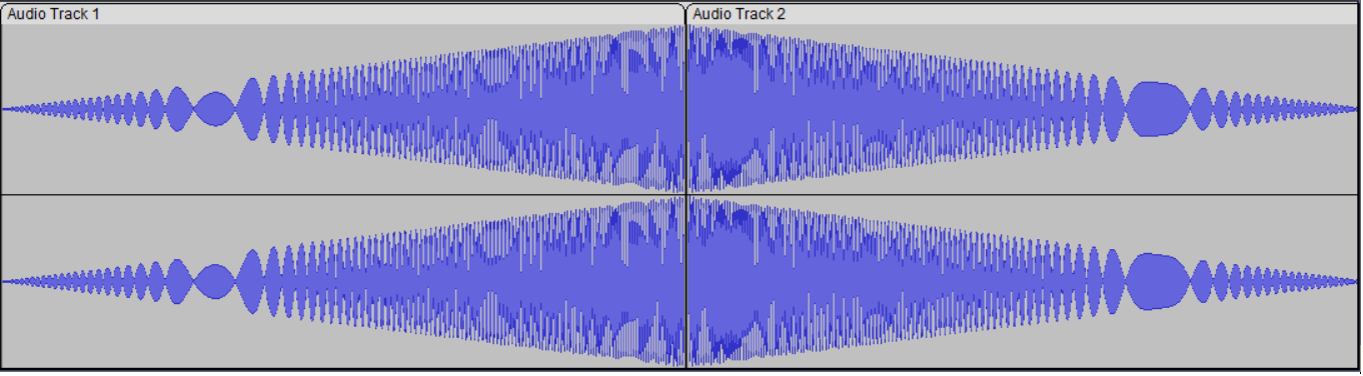
\includegraphics[width=0.8\textwidth]{sprz/wykres_fali}
    \caption{Wykres fali dźwiękowej}
    \label{img:wykres_fali}
\end{figure}

Uzyskany w ten sposób wykres fali dźwiękowej skopiowano dziesięciokrotnie i utworzono sekwencję 500 ms dźwięków, przed którą i po której wprowadzono 500 ms ciszy w celu łatwiejszego wyodrębnienia dźwięków po ich późniejszym zarejestrowaniu (\ref{img:wykres_fali_wielokrotnej}).

\begin{figure}[h]
    \centering
    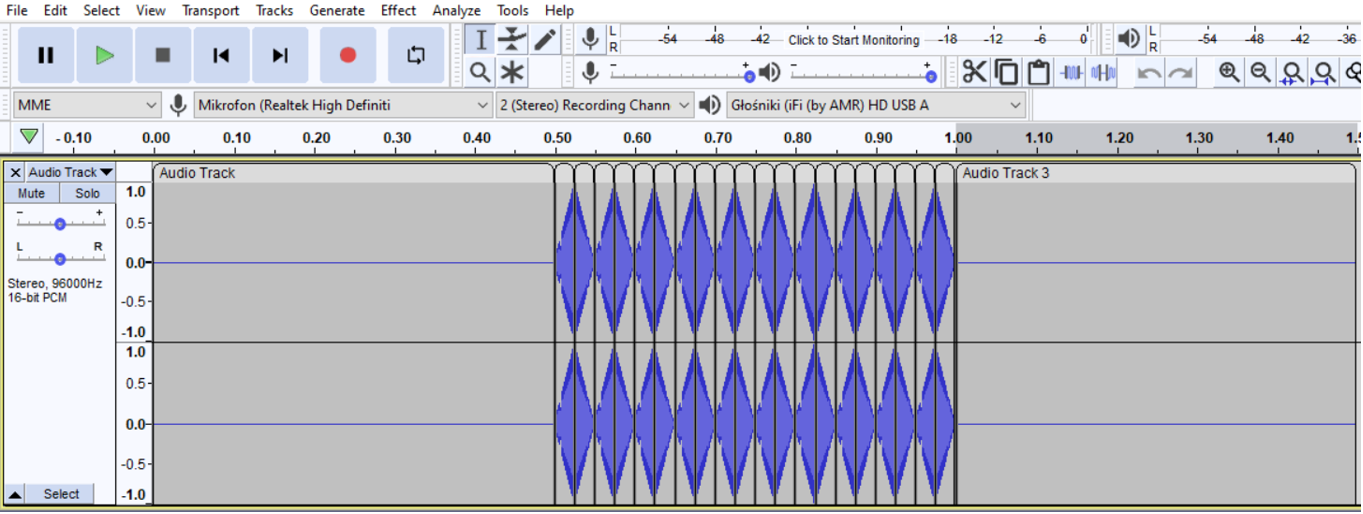
\includegraphics[width=0.8\textwidth]{sprz/wykres_fali_wielokrotnej}
    \caption{Zwielokrotniony wykres fali}
    \label{img:wykres_fali_wielokrotnej}
\end{figure}

Następnie, do wyemitowania dźwięku doświadczenia niezbędne były urządzenia obsługujące co najmniej dwukrotnie wyższą częstotliwość niż emitowane dźwięki. W tym celu do komputera służącego jako generator dźwięku podłączono wzmacniacz iFi Zen Dac o maksymalnej częstotliwości odtwarzania 384 kHz oraz głośnik ultradźwiękowy Pettersson L400 (10-110 kHz). Do zarejestrowania wyemitowanego dźwięku posłużył mikrofon Pettersson M500-384 o częstotliwości próbkowania 384 kHz.

Program BatSound dołączony do mikrofonu posłużył do wizualizacji zarejestrowanego dźwięku.

\begin{figure}[h]
    \centering
    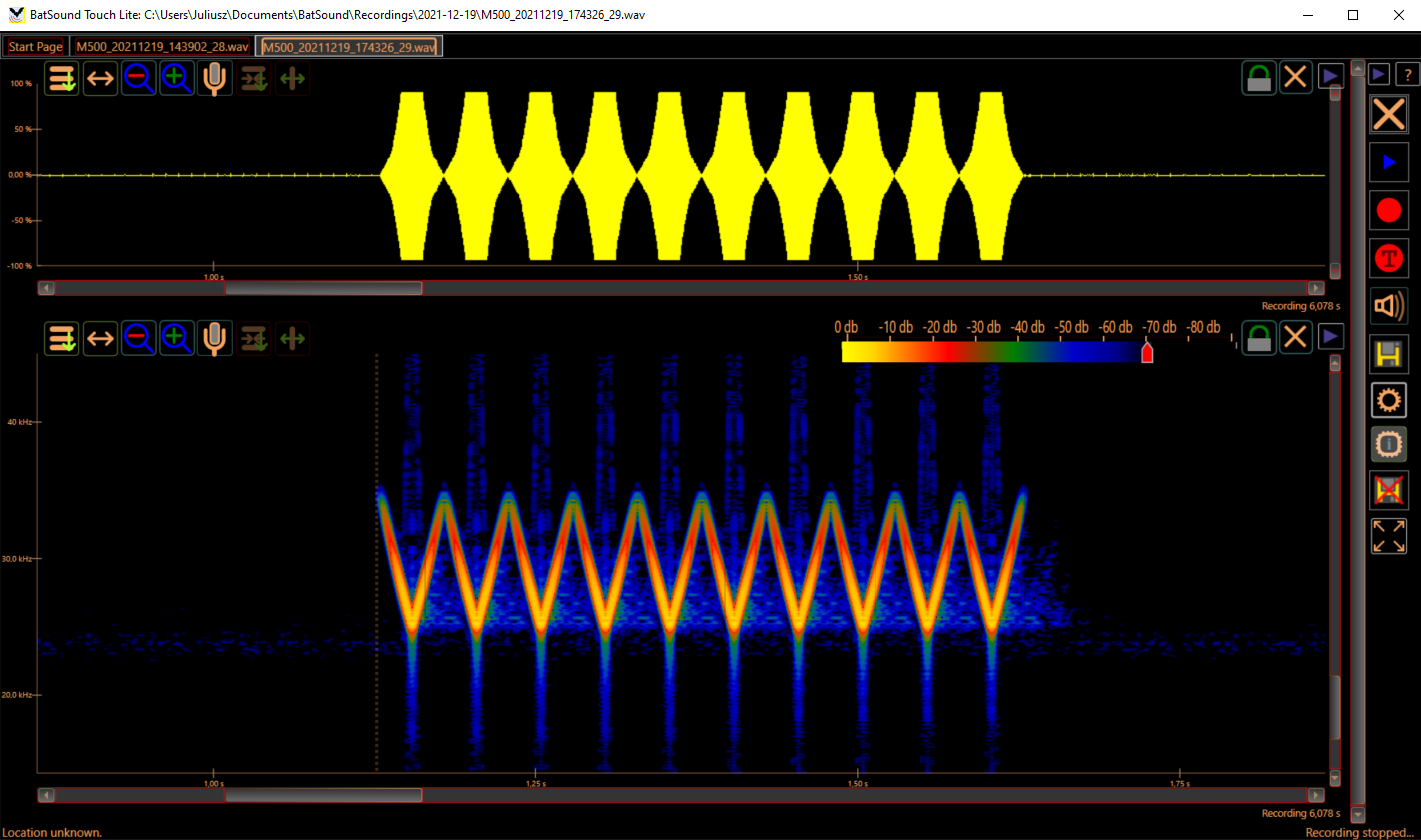
\includegraphics[width=0.8\textwidth]{sprz/batsound}
    \caption{Wykres zarejestrowanego dźwięku zwizualizowany w programie Batsound}
    \label{img:batsound}
\end{figure}

Powyższe doświadczenie dowiodło, iż mikrofon Pettersson M500-384 spełnia swoje zadanie. Mikrofon rejestruje dźwięki w zakresie niesłyszalnym dla człowieka i poprawnie wizualizuje zarejestrowane nagranie.

\subsection{Zebranie nagrań nietoperzy}

\chapter{Struktura produktu}

Struktura wytworzonego produktu została przedstawiona w podziale na poszczególne komponenty.

\section{Architektura systemu}

Na poniższych modelach przedstawiono najważniejsze elementy logiczne, urządzenia wejścia-wyjścia oraz obieg informacji w systemie (\ref{img:model_architektury}). W celu ułatwienia zrozumienia osadzenia systemu w rzeczywistości, architekturę zobrazowano również w postaci graficznej, łącznie z widokiem interfejsu (\ref{img:reprezentacja_graficzna}). 

\begin{figure}[h]
    \centering
    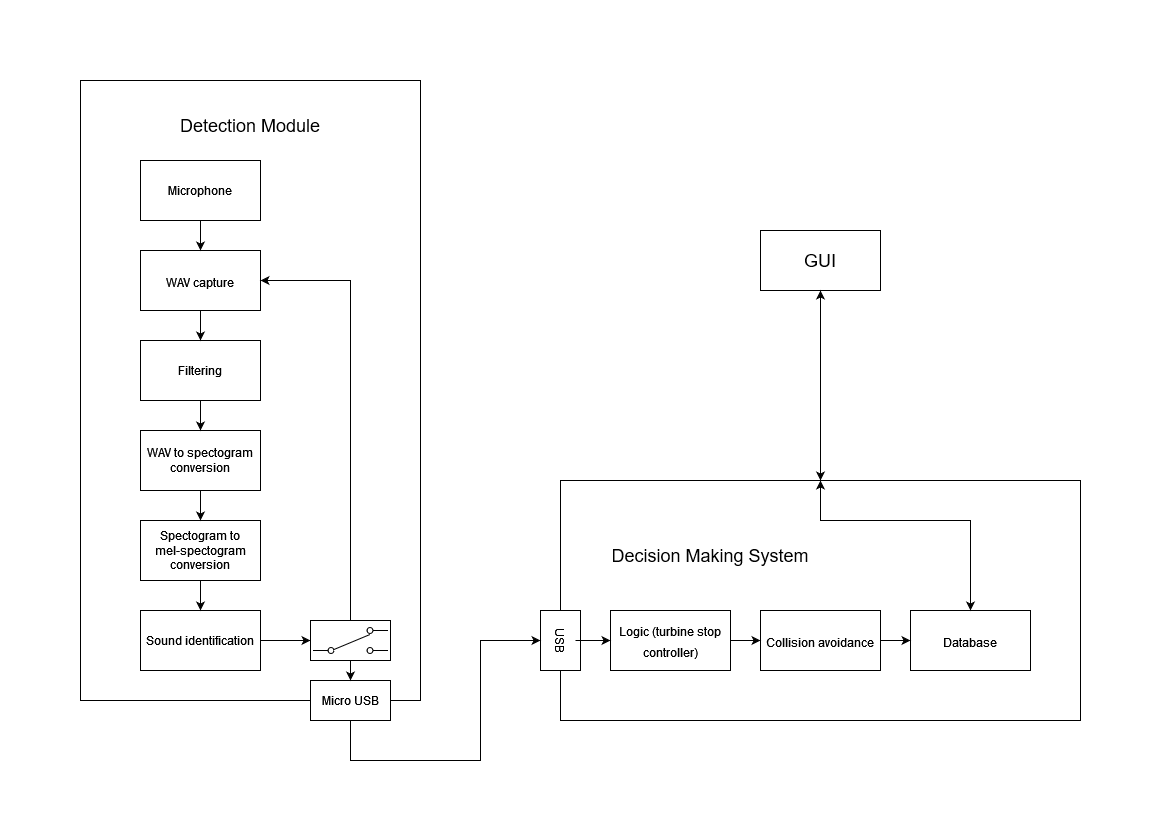
\includegraphics[width=0.8\textwidth]{sprz/model_architektury}
    \caption{Logiczny model architektury systemu}
    \label{img:model_architektury}
\end{figure}

\begin{figure}[h]
    \centering
    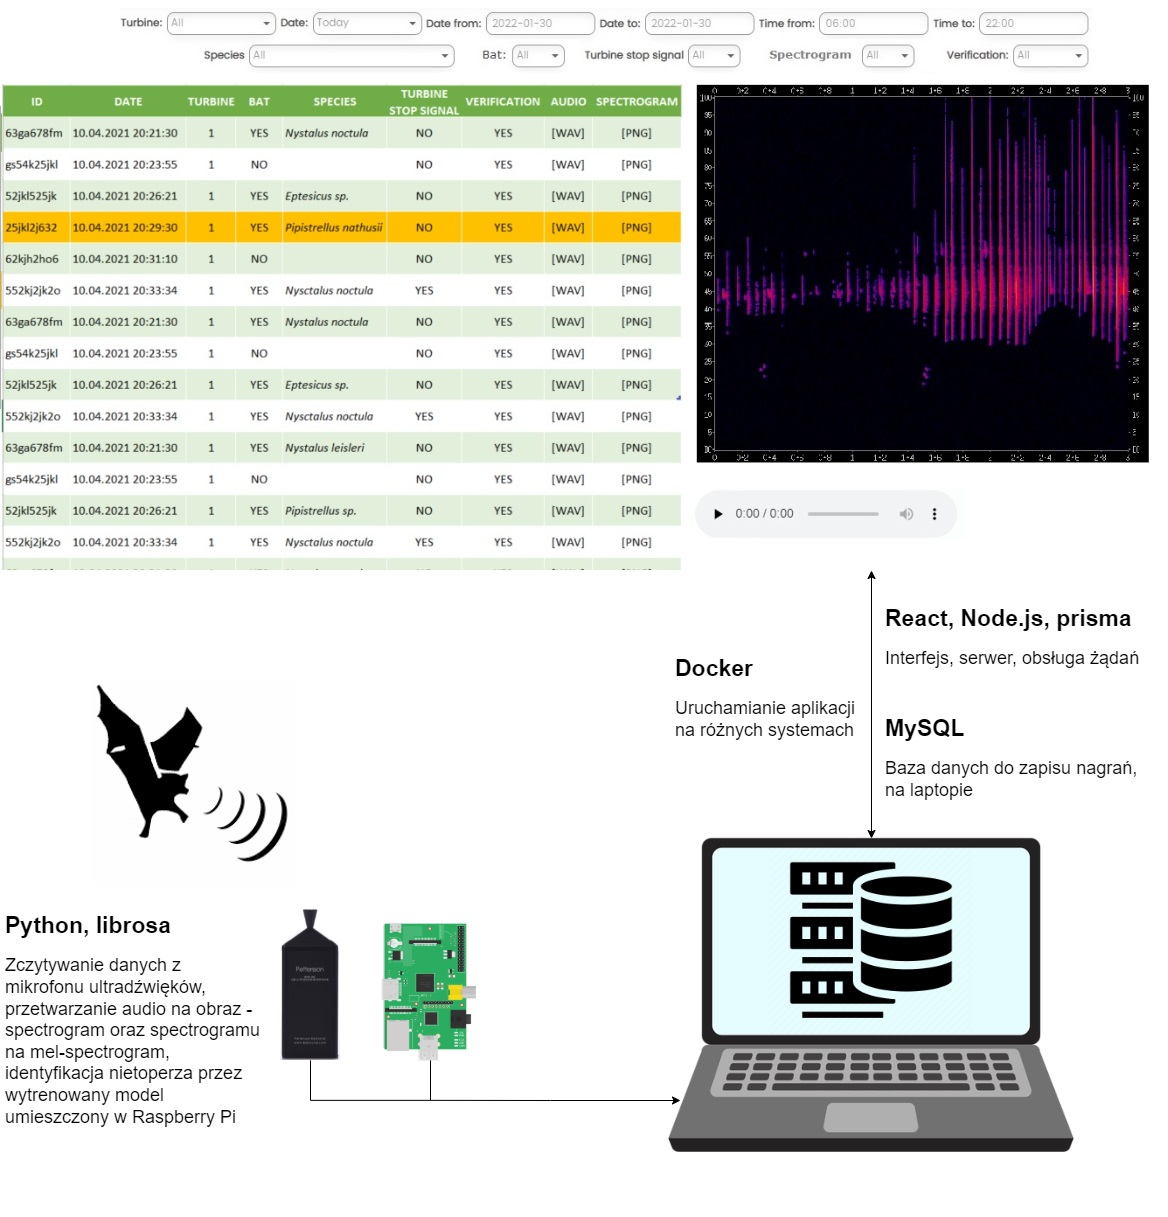
\includegraphics[width=0.8\textwidth]{sprz/reprezentacja_graficzna}
    \caption{Graficzna reprezentacja architektury systemu}
    \label{img:reprezentacja_graficzna}
\end{figure}

\section{Hardware}

\section{Platforma pobierająca i przetwarzająca nagrania z mikrofonu ultradźwięków}

\section{Model sieci neuronowej}

\section{Baza danych}

\section{Aplikacja użytkownika}

\chapter{Realizacja sieci neuronowej}

\section{Przygotowanie danych}

\subsection{Czyszczenie}

\subsection{Dobór typu spektogramu}

\subsection{Cięcie}

\subsection{Augmentacja}

\section{Dobór sieci neuronowej}

\subsection{Przegląd literatury}

\subsection{Konsultacje}

\section{Dobór parametrów sieci neuronowej}

\subsection{Funkcje aktywacji}

\subsection{Funkcja błędu}

\subsection{Optymalizatory}

\subsection{Regularyzacja}

\subsection{Parametry warstw sieci}

\subsection{Transfer learning}

\section{Skuteczność sieci neuronowej}

\subsection{Macierz pomyłek}

\subsection{Metryki}

\subsection{Learning rate}

\chapter{Realizacja interfejsu użytkownika i bazy danych}

\section{Implementacja interfejsu użytkownika}

\section{Implementacja bazy danych}

\chapter{Testowanie}

\section{Testy terenowe produktu}

\section{Testy oprogramowania}

\subsection{Testy jednostkowe}

\subsection{Testy integracyjne}

\subsection{Testy funkcjonalne}

\subsection{Testy akceptacyjne}

\chapter{Przyszłość produktu i komercjalizacja}

\chapter{Podsumowanie}

\chapter{Wkład własny}

\section{Juliusz Orłowski}

\subsection{Wytworzenie sztucznego głosu nietoperza}

\subsection{Interfejs użytkownika}

\subsection{Baza danych}

\subsection{Książka projektu}

\section{Jakub Prucnal}

\subsection{Interfejs użytkownika}

\subsection{Baza danych}

\subsection{Przygotowanie danych do modelu}

\subsection{Model sieci neuronowej}

\subsection{Książka projektu}

\section{Magdalena Wybraniec}

\subsection{Zebranie nagrań nietoperzy}

\subsection{Interfejs użytkownika}

\subsection{Baza danych}

\subsection{Konsultacje chiropterologiczne}

\subsection{Przygotowanie danych do modelu}

\subsection{Model sieci neuronowej}

\subsection{Książka projektu}

\chapter{Załączniki}

\section{Dokument założeń wstępnych}

\begin{documenttable}[]
  \projectname{Batmonit}
  \customer{Bioseco S.A.}
  \contractor{PJATK}
  \projectteam{
    \begin{enumerate}
      \item Juliusz Orłowski
      \item Jakub Prucnal
      \item Magdalena Wybraniec
    \end{enumerate}
  }
  \projectlead{
    \begin{enumerate}
      \item Dawid Gradolewski
    \end{enumerate}
  }
  \documentname{Dokument Założeń Wstępnych}
  \documentowner{Jakub Prucnal}
  \projectsupervisor{dr Tadeusz Puźniakowski}
\end{documenttable}
\begin{center}
  \begin{tabular}{ |p{0.1\linewidth}|p{0.28\linewidth}|p{0.2\linewidth}|p{0.24\linewidth}|p{0.12\linewidth}| }
    \hline
    \multicolumn{5}{|c|}{\textbf{Historia dokumentu}} \\
    \hline
    \textbf{Wersja} & \textbf{Opis modyfikacji} & \textbf{Rozdział/strona} & \textbf{Autor modyfikacji} & \textbf{Data}\\
    \hline
    {1.0} & {Wstępna wersja} & {Całość} & {Magdalena Wybraniec \newline Jakub Prucnal} & {2021-11-21}\\
    \hline
    {2.0} & {Rozbudowanie opisu problemu, doprecyzowanie i drobne korekty pozostałych elementów} &
    {Całość} & {Magdalena Wybraniec} & {2021-12-14}\\
    \hline
  \end{tabular}
\end{center}

\begin{enumerate}[label=\textbf{\arabic*}.]
  \item \textbf{Opis problemu}
  
    Farmy wiatrowe mogą mieć znaczący wpływ na środowisko naturalne, w szczególności nietoperze. Wszystkie gatunki nietoperzy w Polsce są objęte ścisłą ochroną gatunkową i podlegają ochronie prawnej zgodnie z Rozporządzeniem Ministra Środowiska z dnia 16 grudnia 2016 r. w sprawie ochrony gatunkowej zwierząt. Tym samym inwestor realizujący inwestycję wiatrową przestrzegając prawa ochrony przyrody jest zobligowany uzyskać tzw. Decyzję Środowiskową (dalej: DŚ). Zawarte są w niej wszelkie informacje dotyczące:
    \begin{itemize}
      \item chiropterofauny danego obszaru zebrane w trakcie rocznego monitoringu przedrealizacyjnego,
      \item szacowanego wpływu inwestycji na nietoperze,
      \item działań zapobiegających i minimalizujących ewentualny wpływ inwestycji na nietoperze, tak by spełniała ona założenia dobrych praktyk i przepisy prawa – polskiego i międzynarodowego.
    \end{itemize}

    Dotychczas przyjętą praktyką w przypadku wykrycia zbyt dużych aktywności nietoperzy w monitoringu przedrealizacyjnym było wpisanie do DŚ obowiązkowych wyłączeń turbin w okresach, w których te zbyt duże aktywności wykryto. Jednak aktywność nietoperzy jest bardzo zmienna i po realizacji inwestycji niekoniecznie nietoperze będą w całych tych okresach aktywne na farmie, a przez to zagrożone. A wyłączenia turbin na całe długie okresy w roku wiążą się z ogromnymi stratami inwestorów. System opracowany w ramach niniejszej pracy inżynierskiej mógłby zapoczątkować nowe standardy na poziomie krajowym, europejskim i światowym, w zakresie niezbędnych działań minimalizujących wpływ wiatraków na nietoperze - zamiast dotychczas stosowanych z góry określonych wyłączeń na długi okres, można by stosować wyłączenia sterowane na bieżąco systemem – turbiny wyłączane by były tylko w czasie, kiedy większe liczby nietoperzy faktycznie się pojawiają.

    Problem ten dotyczy głównie farm lądowych, gdyż na farmach morskich aktywność nietoperzy jest zdecydowanie mniejsza.

    Zaprojektowany w ramach pracy inżynierskiej system ma za zadanie wytworzenie prototypu urządzenia zczytującego głos nietoperzy z mikrofonu ultradźwięków i ich analizę, tak by automatycznie wykrywać wystąpienie przelotu nietoperzy przy użyciu narzędzi sztucznej inteligencji, takich jak machine learning (dalej: ML) lub deep learning (dalej DL).

    Głównym udziałowcem i zarazem pomysłodawcą jest firma BIOSECO, której przedstawicielami są Dawid Gradolewski oraz Damian Dziak. Udziałowcami produktu, który może zostać wytworzony na dalszym etapie na bazie projektu inżynierskiego, są inwestorzy przygotowujący farmy wiatrowe w Polsce i na świecie, takie jak PGE, Energa, RWE, Polenergia, Iberdrola itd., a także twórcy monitoringów chiropterologicznych, Regionalne i Generalna Dyrekcja Ochrony Środowiska - posiadający tę opcję działań minimalizujących w swoim w arsenale.

    \begin{figure}[h]
        \centering
        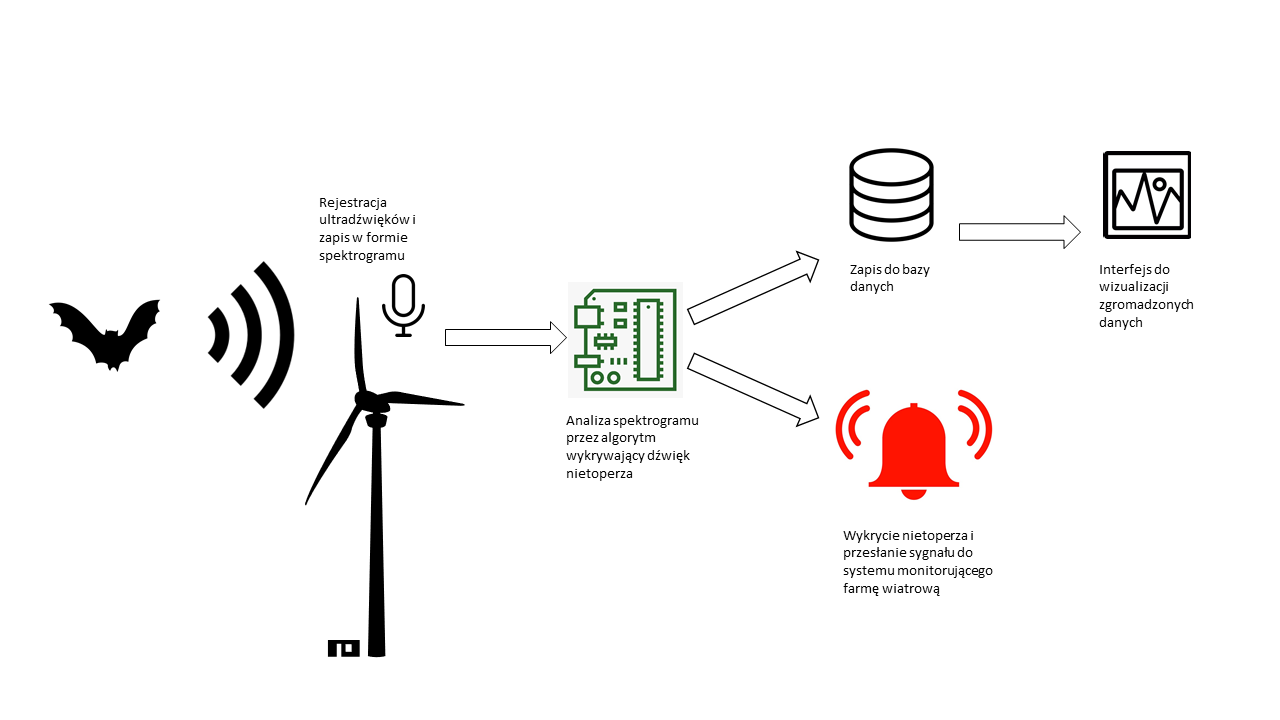
\includegraphics[width=0.8\textwidth]{sprz/rich_picture}
        \label{img:rich_picture}
    \end{figure}

  \item \textbf{Cele systemu}
  
    System ma na celu zczytywać z mikrofonu ultradźwięki wydawane przez nietoperze, przesyłać je do uprzednio wytrenowanego modelu i sygnalizować, gdy nietoperze się pojawią, podając przy tym wykryty gatunek. Jednocześnie powinien zapisywać sygnały nietoperzy w bazie danych i wizualizować je w interfejsie użytkownika.  System po dopracowaniu i ewentualnej komercjalizacji przeznaczony będzie głównie dla firm posiadających lub zarządzających dużymi farmami wiatrowymi. Korzyści wynikające z zastosowania systemu to: ograniczenie śmiertelności nietoperzy na farmach wiatrowych i możliwość zrealizowania zapisów wynikających z pozwoleń prawnych na realizację konkretnego przedsięwzięcia.

  \item \textbf{Kontekst systemu}
  
    System będzie składał się z mikrofonu ultradźwięków wraz z urządzeniem rejestrującym dźwięk (komputerem), do którego będą trafiały wszystkie nagrania, tam analizowane i wystawiające API dla systemu wyłączającego turbinę wiatrową - zamontowane na turbinie wiatrowej.

  \item \textbf{Zakres systemu (funkcjonalność)}
  
    Do głównych funkcjonalności systemu będą należały:

    \begin{itemize}
      \item Rejestracja nagrań,
      \item Przesyłanie nagrań do urządzenia wewnętrznego, na którym są one przechowywane, analizowane i wstawiane do modelu ML/DL,
      \item Analiza nagrań z udziałem modelu ML/DL pod kątem występowania nietoperzy i ich gatunków,
      \item Wizualizacja nagrań nietoperzy w bazie danych poprzez interfejs, wraz z możliwością ich szczegółowego przeglądania.
    \end{itemize}

  \item \textbf{Wymagania jakościowe i inne}
  
    System powinien spełniać następujące wymagania:

    \begin{itemize}
        \item Przenośność urządzenia zewnętrznego,
        \item Niezawodne zasilanie urządzenia zewnętrznego,
        \item Adekwatna do warunków środowiskowych i technologicznych obudowa urządzenia zewnętrznego,
        \item Niezawodność połączenia pomiędzy zewnętrznym urządzeniem rejestrującym nagrania i urządzeniem przechowującym je,
        \item Możliwość wystawienia API i wykorzystania przez system wyłączający i włączający turbinę wiatrową.
    \end{itemize}

  \item \textbf{Wizja konstrukcyjna}
  
    Urządzenie zewnętrzne będzie składało się z mikrofonu Pettersson M500-384 (i opcjonalnie z obudową) oraz urządzenia rejestrującego nagranie (np. Raspberry Pi, komputer - do ustalenia), wyposażonego w zasilanie i pamięć. Kod pobierający nagranie z mikrofonu do urządzenia rejestrującego będzie utworzony pierwotnie w Pythonie. Kod modelu ML/DL będzie napisany w Pythonie z użyciem frameworka TensorFlow, PyTorch, lub innego.  

  \item \textbf{Ograniczenia}
  
    \begin{itemize}
      \item Czas trwania projektu jest ograniczony do momentu przekazania książki dyplomowej do dziekanatu uczelni PJATK.
      \item Ograniczona dostępność nagrań głosów nietoperzy w full-spectrum – możliwa sytuacja, gdy tworzenie projektu będzie odbywało się na podstawie nagrań przetworzonych.
      \item Aktywność nietoperzy ma miejsce od końca marca do października – w związku z tym brak możliwości nagrywania ich aktywności w trakcie semestru zimowego – a tym samym brak możliwości wykonania prób hardware’u przed kwieniem 2022.
    \end{itemize}

  \item \textbf{Słownik pojęć}
  
    Nagranie full-spectrum – nagranie rejestracji ultradźwięków w pełnym wymiarze

    ML (machine learning, uczenie maszynowe) – obszar sztucznej inteligencji wykorzystujący algorytmy i modele matematyczne, które automatycznie poprawiają się poprzez ekspozycję na dane, w celu prognozowania lub podejmowania decyzji dot. nowo dostarczanych danych

    DL (deep learning) – podzbiór ML wykorzystujący tzw. sieci neuronowe, w której pojedyncze neurony tworzą warstwy i stanowią de facto mnożenie wartości wejściowych z początkowo losowo przypisanymi wagami, gdzie wyniki z poszczególnych wejść są sumowane i przekazywane do tzw. funkcji aktywacji, które decydują czy i jakie wyniki przekazać do kolejnej warstwy neuronów.

\end{enumerate}

\section{Specyfikacja wymagań systemowych}

\begin{documenttable}[]
  \projectname{Batmonit}
  \customer{Bioseco S.A.}
  \contractor{PJATK}
  \projectteam{
    \begin{enumerate}
      \item Juliusz Orłowski
      \item Jakub Prucnal
      \item Magdalena Wybraniec
    \end{enumerate}
  }
  \projectlead{
    \begin{enumerate}
      \item Dawid Gradolewski
    \end{enumerate}
  }
  \documentname{Specyfikacja Wymagań Systemowych}
  \documentowner{Jakub Prucnal}
  \projectsupervisor{dr Tadeusz Puźniakowski}
\end{documenttable}
\begin{center}
  \begin{tabular}{ |p{0.1\linewidth}|p{0.28\linewidth}|p{0.2\linewidth}|p{0.24\linewidth}|p{0.12\linewidth}| }
    \hline
    \multicolumn{5}{|c|}{\textbf{Historia dokumentu}} \\
    \hline
    \textbf{Wersja} & \textbf{Opis modyfikacji} & \textbf{Rozdział/strona} & \textbf{Autor modyfikacji} & \textbf{Data}\\
    \hline
    {1.0} & {Wstępna wersja} & {Całość} & {Jakub Prucnal} & {2021-12-05}\\
    \hline
    {2.0} & {Całość niektórych punktów, poprawki reszty} & {punkty 2, 2.1, 2.3} & {Magdalena Wybraniec} & {2021-12-19}\\
    \hline
  \end{tabular}
\end{center}

\begin{enumerate}[label=\textbf{\arabic*}.]
  \item \textbf{Wprowadzenie – o dokumencie}
    \begin{enumerate}[font=\bfseries]
      \item \textbf{Cel dokumentu}
      
        Zdefiniowanie wymagań na podstawie analizy otoczenia projektu oraz analizę potrzeb klienta.

      \item \textbf{Zakres dokumentu}
      
        Określenie udziałowców, zdefiniowanie wymagań, analiza otoczenia projektu.

      \item \textbf{Dokumenty powiązane}
      
        Karta Projektu (KP)
        Dokument Założeń Wstępnych (DZW)
        Rich Picture

      \item \textbf{Odbiorcy}
      
        \begin{itemize}
          \item Opiekun projektu Tadeusz Puźniakowski,
          \item Zespół projektowy,
          \item Przedstawiciele zleceniodawcy: Dawid Gradolewski oraz Damian Dziak
          \item Zleceniobiorca
        \end{itemize}  

      \item \textbf{Słownik pojęć}
      
        Nagranie full-spectrum – nagranie rejestracji ultradźwięków w pełnym wymiarze
        ML (machine learning, uczenie maszynowe) – obszar sztucznej inteligencji wykorzystujący algorytmy i modele matematyczne, które automatycznie poprawiają się poprzez ekspozycję na dane, w celu prognozowania lub podejmowania decyzji dot. nowo dostarczanych danych 
        DL (deep learning) – podzbiór ML wykorzystujący tzw. sieci neuronowe, w której pojedyncze neurony tworzą warstwy i stanowią de facto mnożenie wartości wejściowych z początkowo losowo przypisanymi wagami, gdzie wyniki z poszczególnych wejść są sumowane i przekazywane do tzw. funkcji aktywacji, które decydują czy i jakie wyniki przekazać do kolejnej warstwy neuronów.      

    \end{enumerate}
  \item \textbf{Projekt w kontekście}
    \begin{enumerate}[font=\bfseries]
      \item \textbf{Kontekst biznesowy}
      
        \begin{figure}[h]
          \centering
          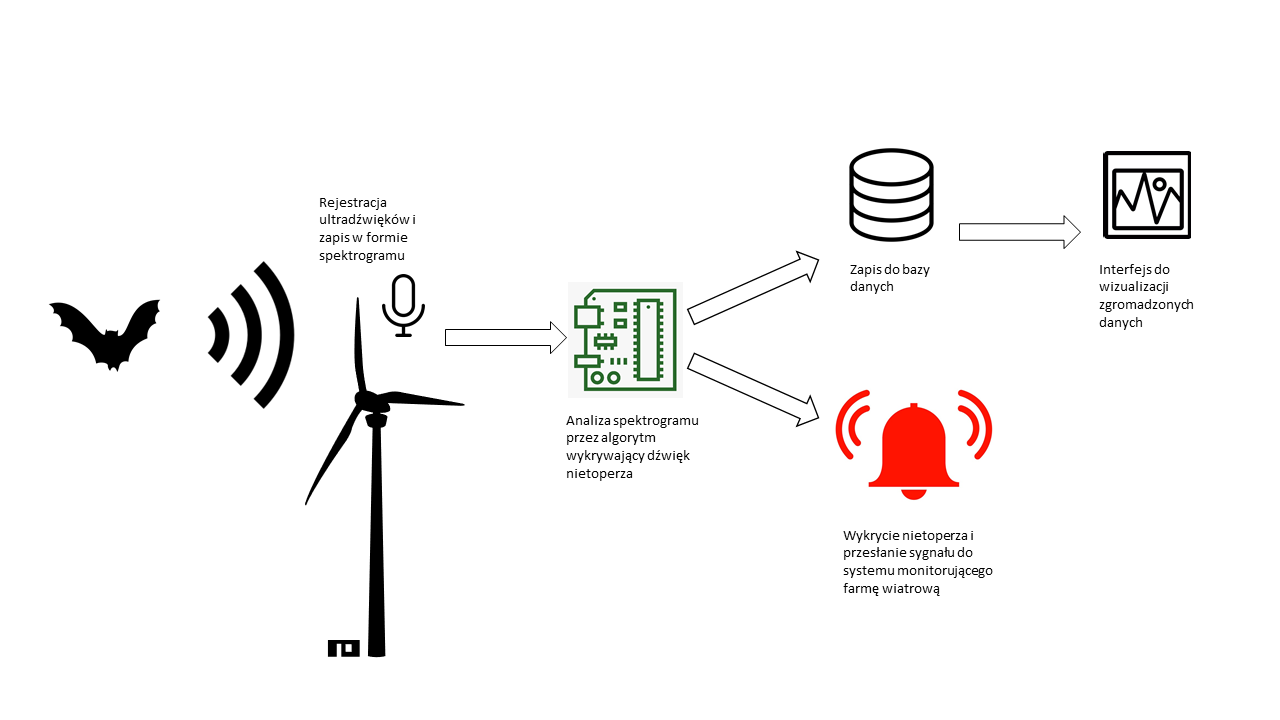
\includegraphics[width=0.8\textwidth]{sprz/rich_picture}
          \label{img:rich_picture}
        \end{figure}

      \item \textbf{Udziałowcy}
      
        \begin{stakeholder}[label={},caption={Klient}][]
          \id{UNB 01}
          \name{Klient}
          \descr{Firma Bioseco}
          \type{Nieożywiony, bezpośredni}
          \viewpoint{Techniczny, ekonomiczny, operatora systemu}
          \limitations{Brak ograniczeń, jest głównym udziałowcem}
          \requ{}
        \end{stakeholder}
        \begin{stakeholder}[label={},caption={Zespół projektowy}]
          \id{UOB 01}
          \name{Zespół projektowy}
          \descr{Zespół deweloperów, którzy tworzą projekt}
          \type{Ożywiony, bezpośredni}
          \viewpoint{Techniczny, wytwórczy}
          \limitations{Nie specyfikuje finansów}
          \requ{}
        \end{stakeholder}
        \begin{stakeholder}[label={},caption={Opiekun projektu}]
          \id{UOP 01}
          \name{Opiekun projektu}
          \descr{dr Tadeusz Puźniakowski}
          \type{Ożywiony, pośredni}
          \viewpoint{Techniczny}
          \limitations{Nie specyfikuje finansów}
          \requ{}
        \end{stakeholder}
        \begin{stakeholder}[label={},caption={Dostarczyciele nagrań nietoperzy}]
          \id{UOP 02}
          \name{Dostarczyciele nagrań nietoperzy}
          \descr{Tribio Sp. z o.o.}
          \type{Ożywiony, pośredni}
          \viewpoint{Ekonomiczny, merytoryczny}
          \limitations{Brak wpływu na aspekty techniczne oprogramowania}
          \requ{}
        \end{stakeholder}
        \begin{stakeholder}[label={},caption={Klienci klienta}]
          \id{UNP 01}
          \name{Klienci klienta}
          \descr{Klienci firmy Bioseco, którzy przesyłają zapytania o produkt do wykrywania nietoperzy}
          \type{Nieożywiony, pośredni}
          \viewpoint{Ekonomiczny, operatora systemu}
          \limitations{Brak wpływu na aspekty techniczne}
          \requ{}
        \end{stakeholder}
        \begin{stakeholder}[label={},caption={Regulacje prawne}]
          \id{UNP 02}
          \name{Regulacje prawne}
          \descr{Regulacje prawne wynikające z prawa ochrony przyrody i prawda dotyczącego ocen oddziaływania na środowisko}
          \type{Nieożywiony, pośredni}
          \viewpoint{Legislacyjny}
          \limitations{Nie specyfikuje finansów}
          \requ{}
        \end{stakeholder}
        \clearpage

      \item \textbf{Klienci}
      
        Klienci wewnętrzni:
        \begin{itemize}
          \item Dziekan
          \item Promotor
        \end{itemize}

        Klienci zewnętrzni:
        \begin{itemize}
          \item Przedstawiciele Bioseco
          \item Przedstawiciele klientów Bioseco potrzebujący urządzenia do wykrywania nietoperzy na farmach wiatrowych by sprostać wymogom prawa ochrony przyrody
          \item Firma Pettersson, producent użytego detektora, wzmacniacza i ich oprogramowania,
          \item Firma Tribio, główny dostawca nagrań nietoperzy do modelu DL
        \end{itemize}

      \item \textbf{Charakterystyka użytkowników}

        \textbf{Administrator} będzie zajmować się testowaniem systemu i zgrywaniem bazy danych uzyskanych w trakcie gdy system jest włączony. Liczebność tego użytkownika znajduje się w przedziale od 1 do 5.

        \textbf{Zwykły użytkownik} będzie zajmował się przeglądaniem i analizą danych z nagrań. Liczebność tego użytkownika znajduje się w przedziale od 1 do 20.

    \end{enumerate}

  \item \textbf{Wymagania}
  
    W niniejszym rozdziale wymienia i opisuje się wymagania narzucone przez klienta - Bioseco, przedstawicieli Uczelni – Dziekana i Promotora, a także przez aktualne standardy prawne dotyczące ochrony przyrody oraz aktualne standardy sprzętowe dotyczące nagrywania i identyfikacji nietoperzy.

    \begin{enumerate}[font=\bfseries]
      \item \textbf{Wymagania ogólne i dziedzinowe}
      
        \begin{requirementstab}[label={tab:requirements:general},caption={Baza danych nagrań głosów nietoperzy}]
          \id{WO 01}
          \priority{M}
          \name{Baza danych nagrań głosów nietoperzy}
          \descr{Zebranie lub pozyskanie bazy danych głosów nietoperzy oraz jej przygotowanie, która posłuży do stworzenia modelu rozpoznawania wystąpienia nietoperza i/lub gatunku nietoperza.}
          \sholder{UOB 01, UOP 01, UNB 01}
          \reqrelated{WO 03}
        \end{requirementstab}
        \begin{requirementstab}[label={tab:requirements:general},caption={Ekologia}]
          \id{WO 02}
          \priority{M}
          \name{Ekologia}
          \descr{System ma chronić nietoperze przed szkodliwym działaniem farm wiatrowych na ich populację}
          \sholder{UNB 01, UNP 01, UNP 02}
          \reqrelated{WO 03}
        \end{requirementstab}
        \begin{requirementstab}[label={tab:requirements:general},caption={Normy prawa}]
          \id{WO 03}
          \priority{M}
          \name{Normy prawa ochrony przyrody i prawa dotyczącego ocen oddziaływania na środowisko}
          \descr{System poprzez swoją przyszłą funkcjonalność wyłączania turbiny będzie stanowił alternatywę dla jedynego obecnie rodzaju działań minimalizujących wpływ turbin na nietoperze, czyli 3 lat monitoringu porealizacyjnego i adekwatnych do jego wyników, narzuconych z góry okresowych wyłączeń turbin, co przyniesie znaczne oszczędności dla deweloperów farm wiatrowych.}
          \sholder{UNP 02}
          \reqrelated{WO 02}
        \end{requirementstab}
        \begin{requirementstab}[label={tab:requirements:general},caption={System rozpoznawania gatunków nietoperzy}]
          \id{WO 04}
          \priority{S}
          \name{System rozpoznawania gatunków nietoperzy}
          \descr{System do rozpoznawania gatunków nietoperzy jest kosztowny, stworzenie go będzie oprogramowaniem, który przyniesie dodatkowe zyski.}
          \sholder{UOB 01, UNB01}
          \reqrelated{}
        \end{requirementstab}
        \clearpage

      \item \textbf{Wymagania funkcjonalne}
      
        \begin{requirementstab}[label={tab:requirements:func1},caption={System przygotowania i normalizacji danych}]
          \id{WF01}
          \priority{M}
          \name{System przygotowania i normalizacji danych}
          \descr{Stworzenie potrzebnych funkcji w programie do oddzielenia odstających próbek i przygotowanie bazy danych do uczenia maszynowego oraz/lub uczenia sieci neuronowych}
          \acceptcrit{Baza danych uczących model oddzielona od próbek odstających i przystosowana do zadanego zadania.}
          \inputdata{}
          \preconditions{}
          \postconditions{}
          \exceptions{}
          \implementation{}
          \sholder{UOB 01}
          \reqrelated{}
        \end{requirementstab}
        \begin{requirementstab}[label={tab:requirements:func1},caption={System rozpoznawania wystąpienia nietoperza}]
          \id{WF02}
          \priority{M}
          \name{System rozpoznawania wystąpienia nietoperza}
          \descr{Opracowanie algorytmu uczenia maszynowego oraz rozpoznawania wystąpienia nietoperza na żywo poprzez śledzenie sygnałów uzyskanych za pomocą urządzenia do detekcji.}
          \acceptcrit{Wytrenowany model do rozpoznawania wystąpienia nietoperzy.}
          \inputdata{}
          \preconditions{}
          \postconditions{}
          \exceptions{}
          \implementation{}
          \sholder{UNB 01, UNP 01}
          \reqrelated{}
        \end{requirementstab}
        \begin{requirementstab}[label={tab:requirements:func1},caption={System uczenia sieci neuronowej}]
          \id{WF03}
          \priority{C}
          \name{System uczenia sieci neuronowej}
          \descr{Opracowanie systemu do uczenia sieci neuronowej rozpoznawania gatunków nietoperzy.}
          \acceptcrit{Stworzony algorytm do tworzenia modelu do rozpoznawania gatunku nietoperza}
          \inputdata{}
          \preconditions{}
          \postconditions{}
          \exceptions{}
          \implementation{}
          \sholder{UOB 01, UOP 01}
          \reqrelated{}
        \end{requirementstab}
        \begin{requirementstab}[label={tab:requirements:func1},caption={System rozpoznawania gatunku nietoperza}]
          \id{WF04}
          \priority{S}
          \name{System rozpoznawania gatunku nietoperza}
          \descr{Opracowanie systemu do rozpoznawania gatunku nietoperza za pomocą detektora.}
          \acceptcrit{Stworzenie modelu oraz połączenie go z urządzeniem do rozpoznawania nietoperzy.}
          \inputdata{}
          \preconditions{}
          \postconditions{}
          \exceptions{}
          \implementation{}
          \sholder{UOB 01}
          \reqrelated{}
        \end{requirementstab}
        \begin{requirementstab}[label={tab:requirements:func1},caption={Interfejs do wizualizacji danych}]
          \id{WF05}
          \priority{M}
          \name{Interfejs do wizualizacji danych}
          \descr{Stworzenie interfejsu do przeglądania danych pobieranych z bazy danych i wizualizacja tych danych.}
          \acceptcrit{Stworzony interfejs działający i spełniający swoją funkcję.}
          \inputdata{}
          \preconditions{}
          \postconditions{}
          \exceptions{}
          \implementation{}
          \sholder{UOB 01}
          \reqrelated{}
        \end{requirementstab}
        \clearpage

      \item \textbf{Interfejs z otoczeniem}
      
        \begin{requirementstab}[label={tab:requirements:func1},caption={System wyłączający wiatraki}]
          \id{WF01}
          \priority{M}
          \name{System wyłączający wiatraki}
          \descr{Połączenie systemu wykrycia nietoperza z systemem wyłączającym wiatraki}
          \acceptcrit{Stworzenie punktu styku, który będzie jako output dawać sygnał do systemu wyłączającego wiatraki.}
          \inputdata{}
          \preconditions{}
          \postconditions{}
          \exceptions{}
          \implementation{}
          \sholder{UNB 01, UNP 01}
          \reqrelated{}
        \end{requirementstab}
        \begin{requirementstab}[label={tab:requirements:func1},caption={Baza danych}]
          \id{WF02}
          \priority{M}
          \name{Baza danych}
          \descr{Połączenie system z bazą danych, która będzie zbierać dane wystąpienia nietoperza}
          \acceptcrit{Stworzenie punktu styku, który będzie jako output dawać sygnał do systemu wyłączającego wiatraki.}
          \inputdata{}
          \preconditions{}
          \postconditions{}
          \exceptions{}
          \implementation{}
          \sholder{UOP 01, UNB 01}
          \reqrelated{}
        \end{requirementstab}
        \clearpage

      \item \textbf{Wymagania pozafunkcjonalne}
      


      \item \textbf{Wymagania na środowisko docelowe}
      


    \end{enumerate}

  \item \textbf{Odwołania do literatury}
\end{enumerate}

\section{Diagram przypadków użycia}

\printbibliography[title={Bibliografia}, heading=bibintoc]




\end{document}
